\documentclass[tikz,border=4pt]{standalone}
\usepackage{tikz}
\usetikzlibrary{positioning,arrows.meta,fit,backgrounds,calc,matrix}

\definecolor{ctrlFill}{HTML}{dae8fc}
\definecolor{ctrlStroke}{HTML}{6c8ebf}
\definecolor{memFill}{HTML}{ffe6cc}
\definecolor{memStroke}{HTML}{d79b00}
\definecolor{calcFill}{HTML}{cce5ff}
\definecolor{calcStroke}{HTML}{4a86e8}
\definecolor{dataFill}{HTML}{d5e8d4}
\definecolor{dataStroke}{HTML}{82b366}
\definecolor{newStroke}{HTML}{b85450}

% Flow-color legend
\definecolor{actColor}{HTML}{c0392b}   % red, activation
\definecolor{wgtColor}{HTML}{2e86de}   % blue, weight
\definecolor{resColor}{HTML}{27ae60}   % green, result
\definecolor{ctlColor}{HTML}{17a2b8}   % cyan, control

\begin{document}
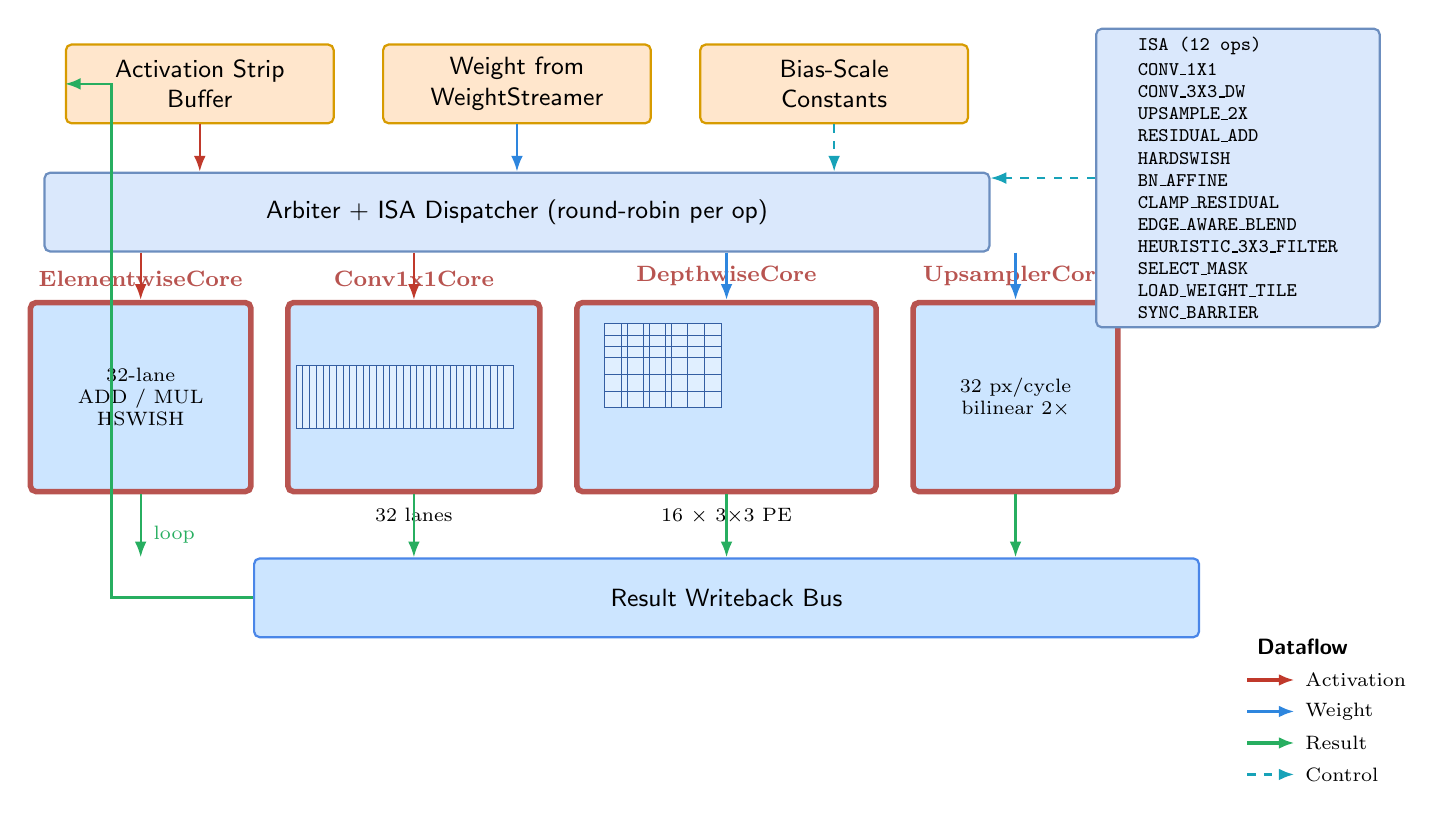
\begin{tikzpicture}[
  font=\small\sffamily,
  mem/.style   ={draw=memStroke,  fill=memFill,  rounded corners=2pt, thick, minimum height=10mm, align=center, inner sep=3pt},
  ctrl/.style  ={draw=ctrlStroke, fill=ctrlFill, rounded corners=2pt, thick, minimum height=10mm, align=center, inner sep=3pt},
  calc/.style  ={draw=calcStroke, fill=calcFill, rounded corners=2pt, thick, minimum height=10mm, align=center, inner sep=3pt},
  core/.style  ={draw=newStroke,  fill=calcFill, rounded corners=2pt, line width=2pt, align=center, inner sep=3pt},
  isa/.style   ={draw=ctrlStroke, fill=ctrlFill, rounded corners=2pt, thick, minimum width=36mm, align=left, inner sep=3pt, font=\scriptsize\ttfamily},
  pe/.style    ={draw=calcStroke!70!black, fill=calcFill!60!white, minimum size=2.2mm, inner sep=0pt, line width=0.3pt},
  lane/.style  ={draw=calcStroke!70!black, fill=calcFill!60!white, minimum width=1.2mm, minimum height=8mm, inner sep=0pt, line width=0.3pt},
  act/.style   ={-{Latex[length=2mm]}, thick, actColor},
  wgt/.style   ={-{Latex[length=2mm]}, thick, wgtColor},
  res/.style   ={-{Latex[length=2mm]}, thick, resColor},
  ctl/.style   ={-{Latex[length=2mm]}, thick, ctlColor, dashed},
  lbl/.style   ={font=\scriptsize, inner sep=1pt},
]

% ==================== Top: sources + arbiter ====================
\node[mem, minimum width=34mm] (abuf) at (0,0)               {Activation Strip\\Buffer};
\node[mem, minimum width=34mm, right=6mm of abuf] (wbuf)     {Weight from\\WeightStreamer};
\node[mem, minimum width=34mm, right=6mm of wbuf] (bsbuf)    {Bias-Scale\\Constants};

\node[ctrl, minimum width=120mm, below=6mm of wbuf] (arb)    {Arbiter + ISA Dispatcher (round-robin per op)};

% ==================== Middle: 4 sub-cores ====================
% ElementwiseCore
\node[core, minimum width=28mm, minimum height=24mm, below=6mm of arb.south west, anchor=north west, xshift=-2mm] (ec) {};
\node[above=0.5mm of ec.north, font=\footnotesize\bfseries, text=newStroke] {ElementwiseCore};
\node[font=\scriptsize, align=center] at (ec.center) {32-lane\\ADD / MUL\\HSWISH};

% Conv1x1Core with 32 vertical lanes
\node[core, minimum width=32mm, minimum height=24mm, right=4mm of ec] (cc) {};
\node[above=0.5mm of cc.north, font=\footnotesize\bfseries, text=newStroke] {Conv1x1Core};
\foreach \i in {0,...,31} {
  \node[lane] at ($(cc.west)+({2mm+\i*0.85mm},0)$) {};
}
\node[font=\scriptsize, below=0.5mm of cc.south, anchor=north] {32 lanes};

% DepthwiseCore with 16x (3x3) PE grid  -> lay out 4 rows x 4 cols of 3x3 blocks
\node[core, minimum width=38mm, minimum height=24mm, right=4mm of cc] (dw) {};
\node[above=0.5mm of dw.north, font=\footnotesize\bfseries, text=newStroke] {DepthwiseCore};
\begin{scope}[shift={($(dw.west)+(3mm,0mm)$)}]
  \foreach \bi in {0,...,3}{
    \foreach \bj in {0,...,3}{
      \pgfmathsetmacro{\bx}{\bi*8}
      \pgfmathsetmacro{\by}{\bj*-4}
      \foreach \i in {0,1,2}{
        \foreach \j in {0,1,2}{
          \node[pe] at ({\bx+\i*2.1 mm + 2mm},{\by + \j*2.1 mm + 4mm}) {};
        }
      }
    }
  }
\end{scope}
\node[font=\scriptsize, below=0.5mm of dw.south, anchor=north] {16 $\times$ 3$\times$3 PE};

% UpsamplerCore
\node[core, minimum width=26mm, minimum height=24mm, right=4mm of dw] (up) {};
\node[above=0.5mm of up.north, font=\footnotesize\bfseries, text=newStroke] {UpsamplerCore};
\node[font=\scriptsize, align=center] at (up.center) {32 px/cycle\\bilinear 2$\times$};

% ==================== Bottom: result writeback + loop arrow ====================
\node[calc, minimum width=120mm, below=8mm of dw.south, anchor=north] (wb) {Result Writeback Bus};

% ==================== Right column: ISA op list ====================
\node[isa, anchor=north west] (isabox) at ($(bsbuf.north east)+(16mm,2mm)$) {%
\textbf{ISA (12 ops)}\\[1pt]
\texttt{CONV\_1X1}\\
\texttt{CONV\_3X3\_DW}\\
\texttt{UPSAMPLE\_2X}\\
\texttt{RESIDUAL\_ADD}\\
\texttt{HARDSWISH}\\
\texttt{BN\_AFFINE}\\
\texttt{CLAMP\_RESIDUAL}\\
\texttt{EDGE\_AWARE\_BLEND}\\
\texttt{HEURISTIC\_3X3\_FILTER}\\
\texttt{SELECT\_MASK}\\
\texttt{LOAD\_WEIGHT\_TILE}\\
\texttt{SYNC\_BARRIER}%
};

% ==================== Arrows ====================
% activations down
\draw[act] (abuf.south) -- (abuf.south |- arb.north);
% weights down
\draw[wgt] (wbuf.south) -- (wbuf.south |- arb.north);
% bias/scale down (control/scale dashed)
\draw[ctl] (bsbuf.south) -- (bsbuf.south |- arb.north);

% arbiter -> each core
\draw[act] (arb.south -| ec.north) -- (ec.north);
\draw[act] (arb.south -| cc.north) -- (cc.north);
\draw[wgt] (arb.south -| dw.north) -- (dw.north);
\draw[wgt] (arb.south -| up.north) -- (up.north);

% cores -> writeback
\draw[res] (ec.south) -- (ec.south |- wb.north);
\draw[res] (cc.south) -- (cc.south |- wb.north);
\draw[res] (dw.south) -- (dw.south |- wb.north);
\draw[res] (up.south) -- (up.south |- wb.north);

% writeback loop -> back to activation strip buffer
\draw[res, line width=1pt] (wb.west) -- ++(-18mm,0) |- (abuf.west);
\node[lbl, text=resColor] at ($(wb.west)+(-10mm,8mm)$) {loop};

% isa dispatcher -> arb (control signal)
\draw[ctl] (isabox.west) -- (isabox.west -| arb.east);

% ==================== Legend (bottom-right) ====================
\begin{scope}[shift={($(wb.east)+(6mm,-4mm)$)}]
  \node[font=\footnotesize\sffamily\bfseries, anchor=north west] (ltitle) at (0,0) {Dataflow};
  \draw[act, line width=1.2pt] ($(ltitle.south west)+(0,-2mm)$) -- ++(6mm,0) node[right, black, font=\scriptsize]{Activation};
  \draw[wgt, line width=1.2pt] ($(ltitle.south west)+(0,-6mm)$) -- ++(6mm,0) node[right, black, font=\scriptsize]{Weight};
  \draw[res, line width=1.2pt] ($(ltitle.south west)+(0,-10mm)$) -- ++(6mm,0) node[right, black, font=\scriptsize]{Result};
  \draw[ctl, line width=1.2pt] ($(ltitle.south west)+(0,-14mm)$) -- ++(6mm,0) node[right, black, font=\scriptsize]{Control};
\end{scope}

\end{tikzpicture}
\end{document}
